\documentclass[article, 1.5space, letterpaper, 12pt, oneside, header, footer]{SydeClass}
\graphicspath{{images/}}
\usepackage{subfigure}
\usepackage{eqnarray}


% --------- Title Info -----------
\titlestyle{design} % used in SydeTitle.tex. Can equal one of the following values: design, work

\title{Lab 1}
\subtitle{Clusters and Classification Boundaries}

\coursecode{SYDE 472}
\department{Systems Design Engineering}

\author{Colin Heics, 20240543}
\authorheader{C. Heics}
\authortwo{Rob Sparrow, 20275155}
\authorheadertwo{R. Sparrow}
\authorthree{Philip Wang, STUNUM}
\authorheaderthree{P. Wang}

\date{\today}
\instructor{Alex Wong}

\subsectionfont{\normalsize}
\setcounter{secnumdepth}{2}
\setcounter{tocdepth}{1}

\input{matlabFormating}

% ############  ############
\begin{document}

% ---------- Title ------------
\input{SydeTitle}

% ############ Chapters ############
\pagenumbering{arabic}

\section{Introduction}
\\This lab investigates three areas: calculating orthonormal transformations, creating decision boundaries using different classification methods, and assessing classification error associated with different methods. All calculations for the purpose of this lab are carried out using the MatLab program.

\\First, data for five separate classes is generated using bivariate Gaussian distribution parameters provided in the lab description. This results in five clusters of two-dimensional data being generated, based on the underlying statistics specified, which is analyzed with respect to the unit standard deviation contour in each class. Analysis of the data is separated into two cases: Case 1 corresponding to the first two classes, and Case 2 corresponding to the remaining three.

\\Next, the cluster data generated is used in development of five separate classification methods to allow for the plotting of decision boundaries in each case. First, the Mean Euclidean Distance (MED), Generalized Euclidean Distance (GED), and Maximum A Posteriori (MAP) methods are implemented and applied to all classes of data. Decision boundaries are plotted for all three methods using data from each of the Cases developed previously, to allow for comparison of the boundaries. Next, the Nearest Neighbor (NN) and Five Nearest Neighbor (5NN) methods are applied to all classes of data. The decision boundaries for both methods are plotted again for the Case 1 and Case 2 sets of classes to allow for comparison.

\\Lastly, the experimental error rate and confusion matrices are developed for each method applied to both Case 1 and Case 2. The experimental error and confusion matrices are analyzed to allow for comparison between the experimental results of each method.

\section{Generating Clusters}

\subsection{Implementation}

\subsection{Results}

\section{Classifiers}

\subsection{Implementation}

\subsubsection{Mean Euclidean Distance}

\subsubsection{General Euclidean Distance}
\\The GED classifier is implemented in a similar manner as the MED classifier. However, in the case of GED a whitening transform is applied to the samples to transform them onto a space where features are both uncorrelated, and have unit-variances. This is accomplished using the weighting matrix W. The distance between two points in the transformed space is calculated as,

\[W=\Lambda^{-1/2}\Phi^{T}\]

\\In the above equation, $\Lambda$ contains the eigen values of the covariance matrix $\Sigma\ as elements, and $\Phi$ contains the eigenvectors of $\Sigma\. After simplification, the distance function is therefore found to be,

\[d_{G}(x,z)= \left [ (x-z)^{T}\Phi\Lambda^{-1/2}\Phi^{T}(x-z) \right ]^{1/2}\]

\\The decision boundary is therefore calculated in the ttwo- and three- class cases as,

\d_{E}\(x,z_{1})=d_{E}\(x,z_{2})
\\left [ (x-z^_{1})^{T}\Phi\Lambda^{-1/2}\Phi^{T}(x-z^_{1}) \right ]^{1/2}\] = \left [ (x-z^_{2})^{T}\Phi\Lambda^{-1/2}\Phi^{T}(x-z^_{2}) \right ]^{1/2}\]
\\left [ (x-z^_{1})^{T}\Phi\Lambda^{-1/2}\Phi^{T}(x-z^_{1}) \right ]^{1/2}\] = \left [ (x-z^_{2})^{T}\Phi\Lambda^{-1/2}\Phi^{T}(x-z^_{2}) \right ]^{1/2}\] = \left [ (x-z^_{3})^{T}\Phi\Lambda^{-1/2}\Phi^{T}(x-z^_3\right ]^{1/2}\]

\\In the case of the MatLab implementation, all points on the grid are classified based on identifying the minimum distance between the point and the mean of each class in the transformed space. This is shown below for both the two- and three- class case,

\min(d_{E}\(x,z_{1}), d_{E}\(x,z_{2}))
\min(d_{E}\(x,z_{1}), d_{E}\(x,z_{2}), d_{E}\(x,z_{3}))

\\This implementation of the GED classifier and method for creating the decision boundary is shown in Appendix A.

\subsubsection{Maximum A Posteriori}

\subsubsection{Nearest Neighbor}

\subsubsection{Five Nearest Neighbor}

\subsection{Results}

\section{Error Analysis}

\section{Conclusions}

\section{Generating Clusters}
Clusters were generated by sampling from a Gaussian distribution, then transforming the samples of each cluster based on the cluster's mean and covariance matrix. The random samples of a standard two-variable Gaussian distribution were generated using MATLAB's $randn()$ function. The samples were then transformed as shown by the example in MATLAB's documentation for $randn()$. The example shows to transform a given vector, x, by the equation
\begin{eqnarray}
\label{eqn:chol_transform}
\underbar{y} = chol \Sigma \underbar{x}+\underbar{\mu}
\end{eqnarray}

where $\underbar{x}$ is a vector in the original space and $\underbar{y}$ is the transformed vector in the new space.

Unit standard deviation contours were also created for each cluster. To find these contours, a vector of points that represented the unit standard deviation contour of a standard two-variable Gaussian distribution was transformed using the previously described transformation method for each cluster.

This method was confirmed to be a viable method for transforming the data by using a second transformation to derive the unit standard deviation contours. The orthonormal covariance transformation shows that vectors of a Gaussian distribution with covarance $\Sigma$ can be transformed to have a covariance of I. This transformation is given by the equation
\begin{eqnarray}
\label{eqn:ortho_transform}
\underbar{x} = {\Lambda}^{-1/2} \Phi^T \underbar{y}
\end{eqnarray}

where columns of $\Phi$ are the eigenvectors of $\Sigma$ and the diagonal elements of $\Lambda$ are the eigenvectors of $\Sigma$. Taking the inverse of this equation and adding the specified mean results in the second transformation for deriving unit standard deviation contours:
\begin{eqnarray}
\label{eqn:ortho_inv_transform}
\underbar{y} = {(\Phi^{T})}^{-1} \Lambda^{-1/2}\underbar{x}+\underbar{\mu}
\end{eqnarray}

Both transformations produced the same unit standard deviation contours.
 
 \subsection{Classes A and B}
 The two classes A and B were characterized by:

\begin{eqnarray}
{\mu}_{A}=\left[ \begin{smallmatrix} 5&10 \end{smallmatrix}\right]^{T} \; & {\Sigma}_{A}=\left[ \begin{smallmatrix} 8&0 \\ 0&4 \end{smallmatrix}\right]^{T} \nonumber\\
{\mu}_{B}=\left[ \begin{smallmatrix} 10&15 \end{smallmatrix}\right]^{T} \; & {\Sigma}_{B}=\left[ \begin{smallmatrix} 8&0 \\ 0&4 \end{smallmatrix}\right]^{T} \nonumber
\end{eqnarray}

\begin{figure}[ht]
\centering
	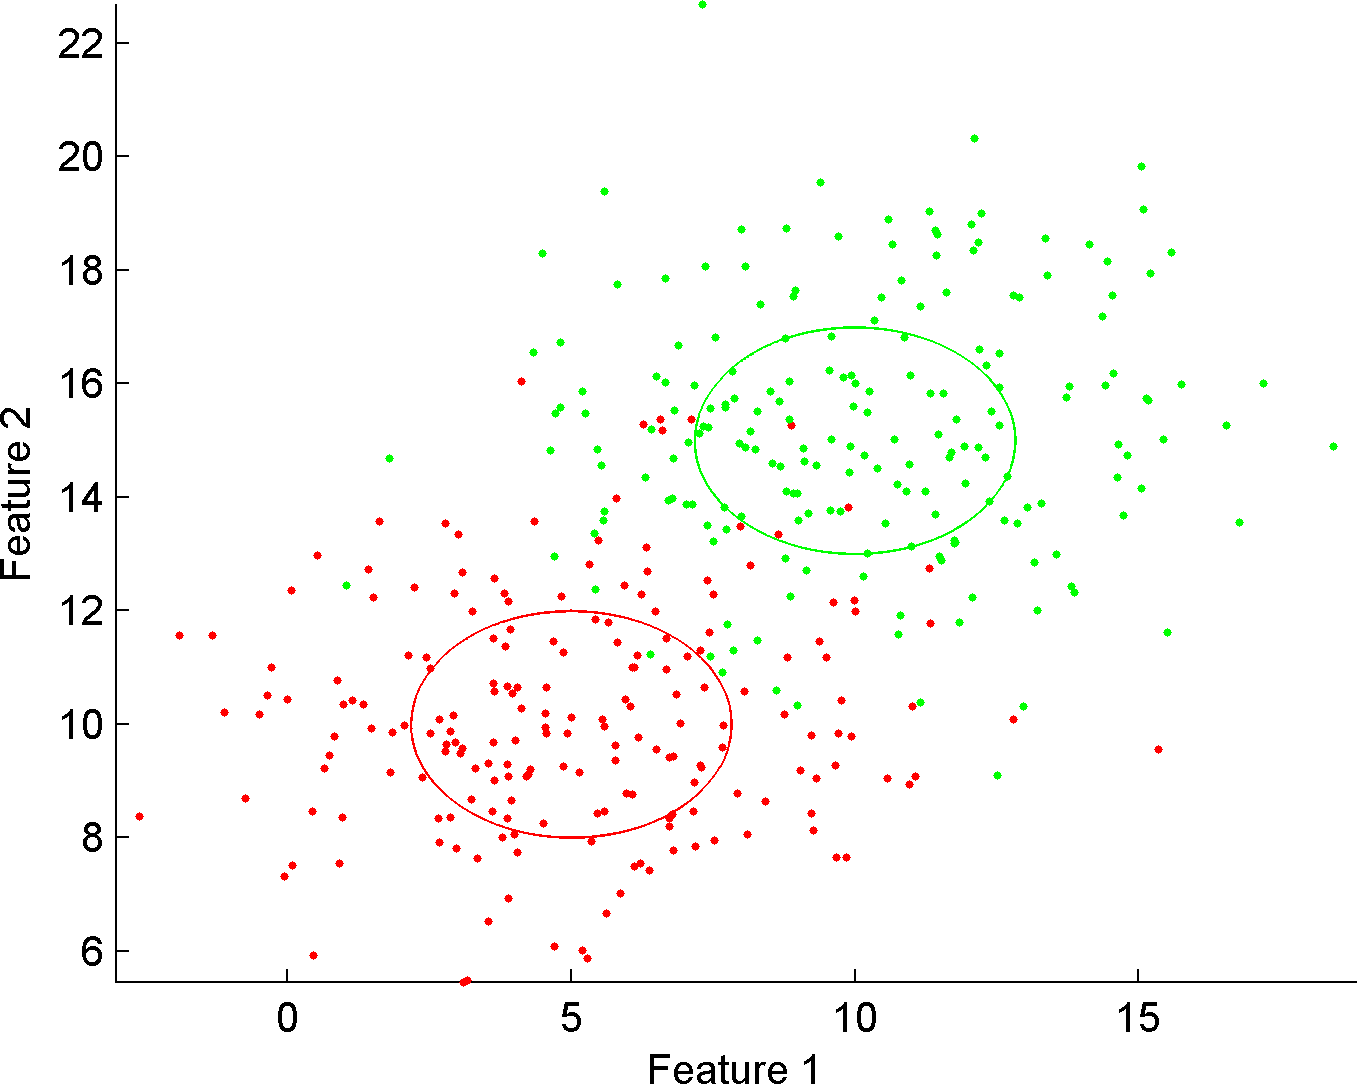
\includegraphics[width=0.9\linewidth]{fig1a-AB_cluster}
	\label{fig:clustersDataAB}
	\caption{Clusters A and B with unit standard deviation elipses}
\end{figure}

 \subsection{Classes C, D, E}
 The three classes C, D and E were characterized by:
 
 \begin{eqnarray}
{\mu}_{C}=\left[ \begin{smallmatrix} 5&10 \end{smallmatrix}\right]^{T} \; & {\Sigma}_{C}=\left[ \begin{smallmatrix} 8&4 \\ 4&40 \end{smallmatrix}\right]^{T} \nonumber\\
{\mu}_{D}=\left[ \begin{smallmatrix} 15&10 \end{smallmatrix}\right]^{T} \; & {\Sigma}_{D}=\left[ \begin{smallmatrix} 8&0 \\ 0&8 \end{smallmatrix}\right]^{T} \nonumber\\
{\mu}_{E}=\left[ \begin{smallmatrix} 10&5 \end{smallmatrix}\right]^{T} \; & {\Sigma}_{D}=\left[ \begin{smallmatrix} 10&-5 \\ -5&20 \end{smallmatrix}\right]^{T} \nonumber
\end{eqnarray}
 
 
\begin{figure}[ht]
\centering
	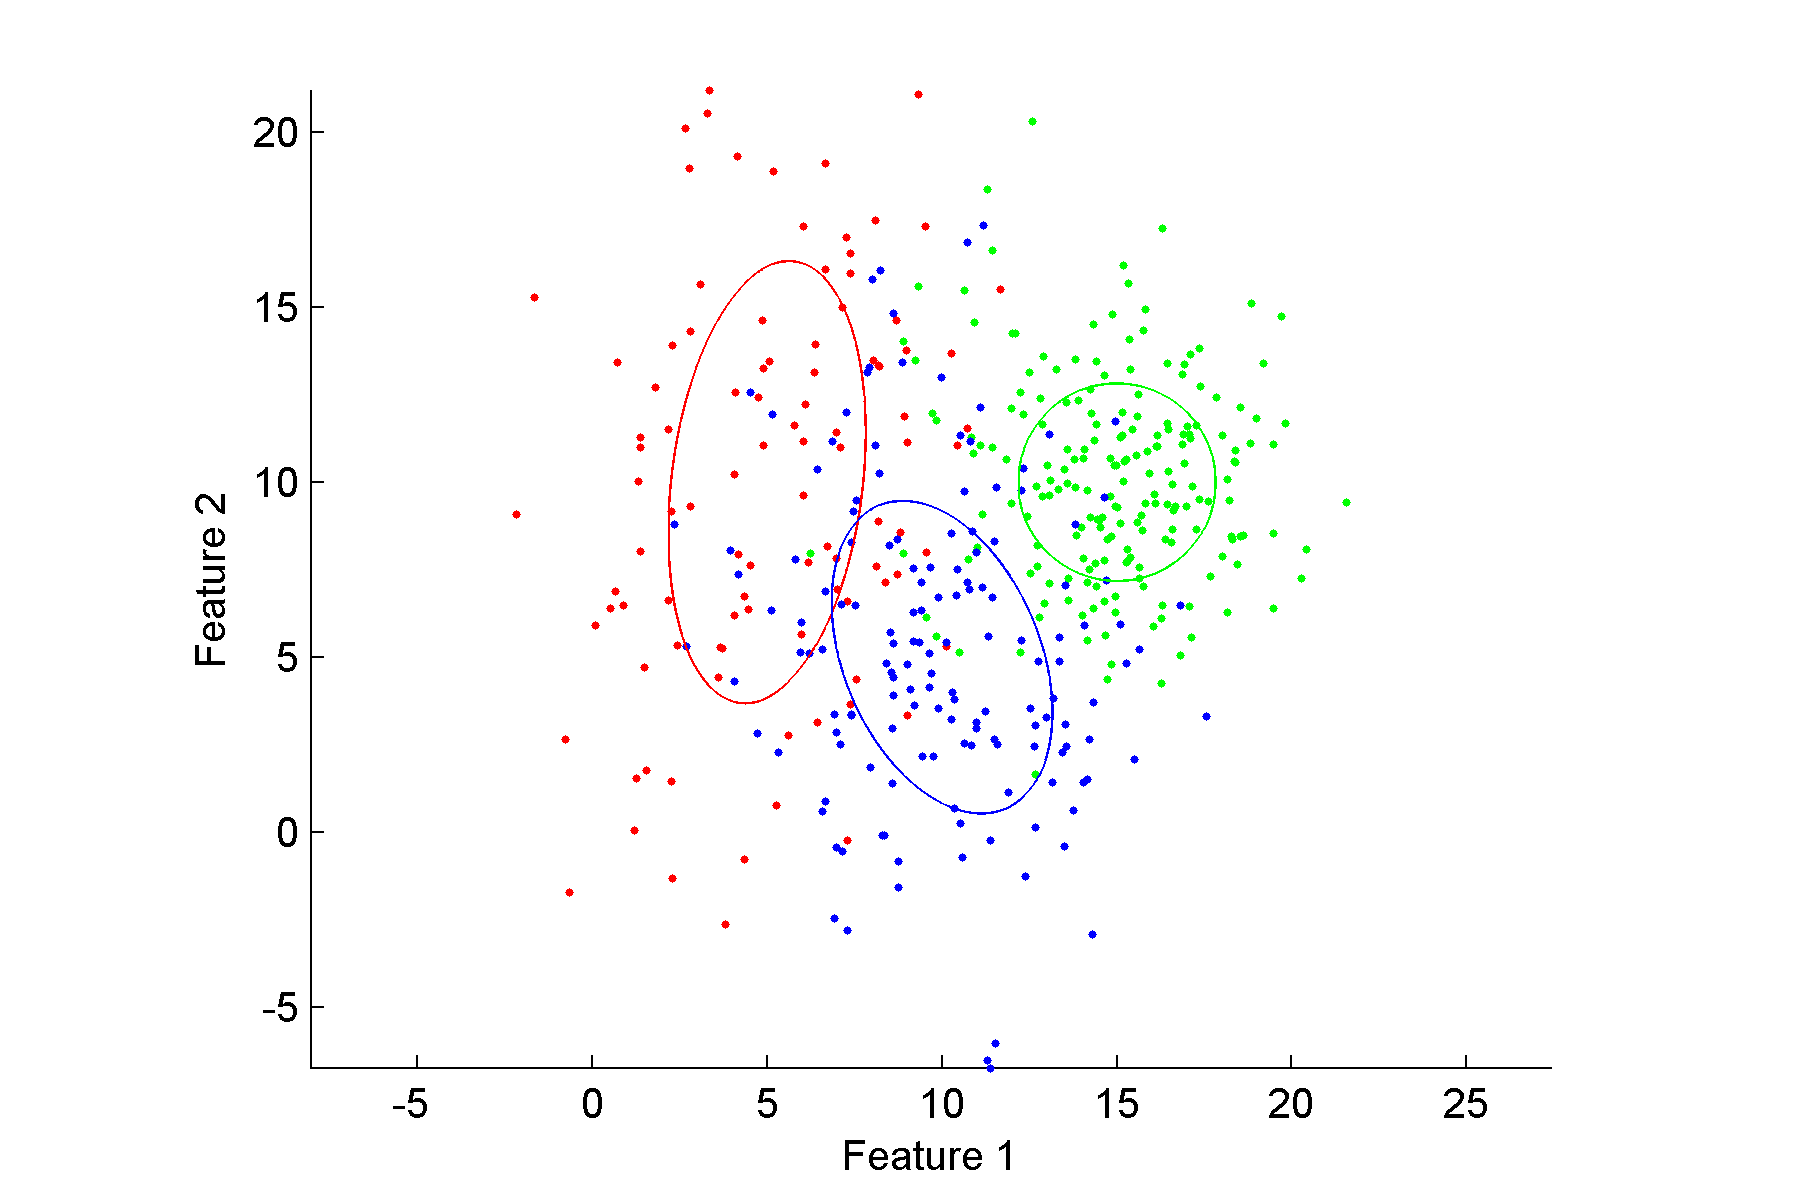
\includegraphics[width=0.9\linewidth]{fig1b-CDE_cluster}
	\label{fig:clustersDataCDE}
	\caption{Clusters C, D, E unit standard deviation elipses}
\end{figure}
 
\clearpage


\appendix
\newpage

\section{Matlab Code}
\subsection{PSNR function}
%\lstinputlisting[language=Matlab]{"matlabFiles/psnr.m"}

\subsection{Chroma Subsampling}
%\lstinputlisting[language=Matlab]{"matlabFiles/lab3_q2.m"}

\subsection{Image Transform}
%\lstinputlisting[language=Matlab]{"matlabFiles/lab3_q3.m"}

\subsection{Quantization}
%\lstinputlisting[language=Matlab]{"matlabFiles/lab3_q2.m"}






% -------- Bibliography --------
%\addcontentsline{toc}{chapter}{\hspace{13pt} References}
\bibliography{refs}

\end{document}  